\documentclass[a4paper,11pt]{article}
\usepackage[latin1]{inputenc}
\usepackage[T1]{fontenc}
\usepackage{bbm} %math chars
\usepackage{amsmath}
\usepackage{indentfirst}
\usepackage{fullpage} %minimizes the default margins
\usepackage{url}
\usepackage{graphicx}
\usepackage[center,footnotesize]{caption} %options des legendes des graphes
\usepackage[section]{placeins} %place les figures d'une section avant le debut de la suivante
\usepackage{subfig} %a) b) c)
\usepackage{ulem} % texte barre
\title{Series 2 - solution}
\date{}
\author{Genomics and bioinformatics - Week 3 - October 2, 2012}
\begin{document}
\maketitle

\section{Overlap graphs}

\begin{enumerate}
\item Just by looking manually at the overlaps (of size 4+):

\begin{center}
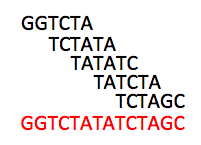
\includegraphics[width=0.3\textwidth]{byhand.png}\\
\end{center}

\item The overlap (Hamiltonian) graph is build by taking the reads as vertices and adding an edge each time two reads have an overlap (of a chosen minimal size, here 4). Then find a path going through every vertex once and only once: this is called an Hamiltonian path. The contig is made of the first read plus, from each read in the path, its sub-sequence (in red below) that does not belong to the overlap. There may be several such paths; the number of them depends on the minimal overlap one chooses.

As in part 1, one finds GGTCTATATCTAGC.

\begin{center}
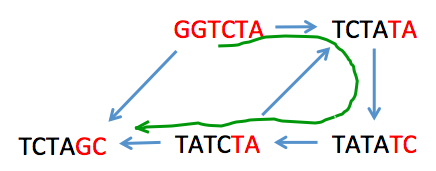
\includegraphics[width=0.5\textwidth]{hamiltonian.png}\\
\end{center}

\item To build the ``De Bruijn'' graph, one proceeds as follows:
	\begin{itemize}
	\item Choose an integer $l$ (here $l=4$ was given). 
	\item Build $S_{l-1}$, the set of all \textit{unique} $l-1$-mers that the reads contain:\\
		$S_{l-1}=$ \{GGT, GTC, TCT, CTA, TAT, ATA, ATC, TAG, AGC\}\\
		These are the vertices of the graph.
	\item Build $S_l$, the set of all $l$-mers that the reads contain:\\
		\begin{tabular}{ll}
		$S_l$ = & \{GGTC, GTCT, TCTA,\\
		              &  TCTA, CTAT, TATA,\\
		              &  TATA, ATAT, TATC,\\
		              &  TATC, ATCT, TCTA,\\
		              &  TCTA, CTAG, TAGC\}
		\end{tabular}
		
		Those are the edges: GGTC binds GGT and GTC, etc. 
	\item Then there are several ways to proceed:
		\begin{itemize}
		\item Some duplicates in $S_l$ are du to the overlaps between reads; some are really a repeat in the sequence of the contig itself. If you have an idea of which ones come from overlaps between reads (as we have here), discard only them. In this case,  
			\begin{tabular}{ll}
		         $S_l$ = & \{GGTC, GTCT, TCTA,\\
		              &  \sout{TCTA}, CTAT, TATA,\\
		              &  \sout{TATA}, ATAT, TATC,\\
		              &  \sout{TATC}, ATCT, TCTA,\\
		              &  \sout{TCTA}, CTAG, TAGC\}
		        \end{tabular}
		        
		        We see that only TCTA is a real repeat.
		\item Use only the unique edges, and artificially double some of the edges if necessary to make the graph Eulerian
		  	(in particular, cyclic, see below).
			Check however that the edges you add are at least among the duplicate reads you decided to discard from $S_l$ when taking only the uniques.
		\item In fact, duplicates are a real problem that is not so easily solved in practice. Real algorithms for example make estimates of the frequency of a repeat in the contig, and allow some errors. 
		\end{itemize}
	\item Close the graph by joining the starting vertex - the only one that has more outgoing than incoming edges - to the end vertex - with more incoming than out coming edges. This should make the graph Eulerian, i.e. cyclic, and every vertex having the same number of incoming and outgoing edges.
	\item Find a cycle that goes through each \textit{edge} once and only once: this is called an Eulerian cycle. The contig is made of the first vertex, plus the last nucleotide of each vertex in the path. 
	
	In the figure below, a green arrow joins the start and end, and the cycle is drawn in red.
		\begin{center}
		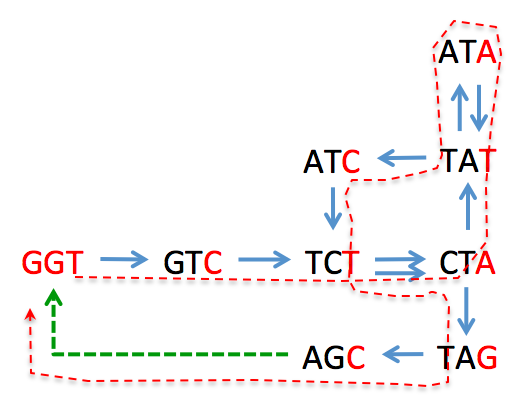
\includegraphics[width=0.5\textwidth]{eulerian.png}\\
		\end{center}
		As in part 1, one finds GGTCTATATCTAGC. Note the TCTA repeat in the sequence.
	\end{itemize}

\end{enumerate}



\end{document}
